\chapter{Architektura i technologie}

Niniejszy rozdział został poświęcony ogólnemu opisowi architektury systemu oraz zastosowanych technologii. Dla poszczególnych wyborów zostały przedstawione przesłanki, którymi kierował się autor tej pracy. 

Istotnym czynnikiem mającym wpływ na wybór technologii oraz wzorców architektonicznych była chęć poszerzenia wiedzy autora niniejszej pracy w ich zakresie. Cechą wspólną wszystkich zastosowanych rozwiązań jest szeroki dostęp do materiałów w postaci dokumentacji oraz pozycji książkowych. 

\section{Architektura systemu}

Ze względu na potrzebę szerokiej dostępności platformy została ona zrealizowana jako system webowy w architekturze klient - serwer. Interfejsem użytkownika końcowego jest aplikacja kliencka typu SPA (ang. \textit{Single Page Application}) uruchamiana w przeglądarce internetowej. Aplikacja ta komunikuje się z API (ang. \textit{Application Programming Interface}) aplikacji serwerowej za pomocą zapytań protokołu HTTP (ang. \textit{Hypertext Transfer Protocol}).  Aplikacja serwerowa z kolei komunikuje się z bazą danych w celu odczytu oraz zapisu informacji za pomocą interfejsu JDBC (ang. \textit{Java DataBase Connectivity}). 

\begin{figure}[ht]
\centering
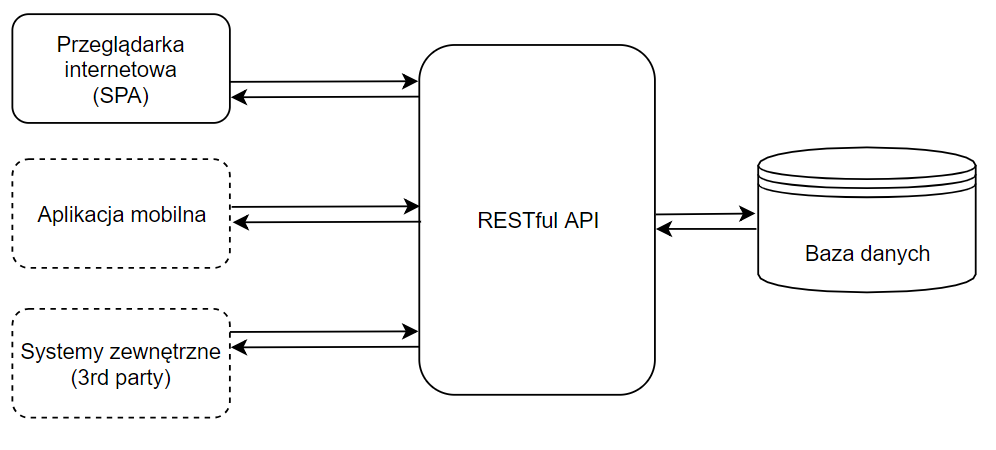
\includegraphics[width=0.8\linewidth]{05-architektura-i-technologie/rys/ogolna-architektura.PNG}
\caption{Diagram ogólnej architektury systemu}
\label{fig:diagram-og-architekt}
\end{figure}

Elementy otoczone linią kreskowaną na diagramie nie są przedmiotem tej pracy, jednak podkreślają uniwersalność API oraz wskazują możliwości rozwojowe oraz integracyjne systemu.

\subsection{RESTful API}
API wystawiane przez część serwerową zostało zaprojektowane w oparciu styl architektoniczny REST (ang. \textit{Representational State Transfer}), który zakłada komunikację klient-serwer z uwzględnieniem następujących zasad: 
\begin{itemize}
\item użycie podstawowych metody protokołu HTTP czyli - GET, PUT, POST oraz DELETE,
\item identyfikacja zasobów poprzez URL (ang. \textit{Uniform Resource Locator}),
\item komunikacja bezstanowa (brak sesji).
\end{itemize}

Użycie podstawowych metod protokołu HTTP pozytywnie wpływa na czytelność oraz intuicyjność API. Projektowanie z uwzględnieniem powyższych zasad pozwala również zminimalizować powiązania pomiędzy serwerem oraz klientem, API staje się uniwersalne. Otwiera to możliwości rozwoju systemu na inne platformy, np. utworzenie aplikacji klienckich dla systemów mobilnych Android oraz iOs. Możliwości rozwoju systemu zostały przedstawione za pomocą zakreskowanych bloków na rysunku~\ref{fig:diagram-og-architekt}

\section{Stos technologiczny}

W poniższych sekcjach zostały przybliżone zastosowane technologie. 

\subsection{Spring Boot}

Aplikacja serwerowa została zaimplementowana w języku Java (w wersji 1.8) \cite{java} z użyciem szkieletu Spring Boot (w wersji 2.0.3) \cite{springboot}. Technologie te zostały wybrane ze względu na następujące czynniki:
 \begin{itemize}
\item rozwiązania open source,
\item duże grono użytkowników oraz baza materiałów w sieci,
\item dobra dokumentacja,
\item duża ilość dostępnych modułów Springa np. do komunikacji z bazami danych,
\item chęć rozwoju autora w zakresie tych technologii.
\end{itemize}

\subsection{JWT}

Technologia JWT (ang.\textit{Json Web Token}) została wybrana jako sposób realizacji autoryzacji zapytań do API systemu. JWT jest technologią autoryzacji bezstanowej, przez co bardzo dobrze współgra z architekturą aplikacji REST-owych.

\subsection{MySQL} 

Relacyjna baza danych została wybrana ze względu na dużą ilość powiązań między encjami w systemie. MySQL od firmy Oracle jest darmowym, bezpiecznym oraz wydajnym systemem zarządzania bazą danych.  Istotnym uzasadnieniem wyboru tej technologii jest również bardzo dobra integracja ze szkieletem Spring.

\subsection{Angular}

Główną technologią wykorzystywaną po stronie front endu jest szkielet do tworzenia SPA (ang. \textit{Single Page Application}) rozwijany przez firmę Google - Angular (w wersji 6.1.0) \cite{angular}. Szkielet ten ułatwia budowę skalowalnych i szybkich aplikacji z bogatym interfejsem użytkownika. Dużą zaletą Angular-a jest wsparcie dla programowania w języku TypeScript, co usprawnia rozwój aplikacji poprzez kontrolę typów.

Dodatkowo w celu usprawnienia procesu rozwoju aplikacji została wykorzystana biblioteka ngrx (w wersji 6.1.0), wspomagająca zarządzanie stanem aplikacji. Wykorzystanie tej biblioteki znacznie ułatwiło analizę działania aplikacji oraz diagnozowanie błędów.


\subsection{AntDesign - NgZorro}

NgZorro zostało użyte jako główna biblioteka dostarczająca szeroką gamę komponentów graficznych do aplikacji w technologii Angular \cite{ngzorro}. Wybór padł na to rozwiązanie ze względu na duże wsparcie dla przeglądarek oraz bardzo dobrą dokumentację z przykładami. Użyte komponenty również cechują się atrakcyjnym wyglądem, który ma duży wpływ na odbiór systemu przez użytkownika.

\subsection{Heroku}

Zaimplementowane aplikacje serwerowa oraz kliencka zostały wdrożone na platformę Heroku. Rozwiązanie to zostało wybrane ze względu na darmowe plany użytkowania, jak również doświadczenie autora pracy w zakresie tej platformy. 
